\documentclass[twocolumn,8pt,b5paper]{extarticle}

%% \Setlength{\textwidth}{17cm}
%% \setlength{\textheight}{24cm}
%% \setlength{\leftmargin}{-0.5cm}
%% \setlength{\topmargin}{-2cm}
%% \setlength{\oddsidemargin}{0cm}
%% \setlength{\evensidemargin}{0cm}

\usepackage{xltxtra}
\setmainfont[Ligatures=TeX]{IPAPMincho}
\setsansfont{IPAPGothic}
\setmonofont{IPAGothic}
\XeTeXlinebreaklocale "ja"

\usepackage{hyperref}
\usepackage{listings}
\lstset{%
 backgroundcolor={\color[gray]{.85}},%
 basicstyle={\small},%
 frame={tb},
 breaklines=true,
 columns=[l]{fullflexible},%
 lineskip=-0.5ex%
}
\usepackage{verbatim}
\usepackage{biblatex}
\addbibresource{ref}
\usepackage{graphicx}
\usepackage{ulem}
\usepackage{myjapanese}

%\usepackage{endnotes}
%\let\footnote=\endnote
\newcommand{\vs}{\vspace{\baselineskip}}

\title{Pietのコード自動生成}
\author{NoNamea 774}

%\renewcommand{\baselinestretch}{0.9}

\begin{document}
\maketitle

\section{なぜこんなものを……。}
ここのサークルの主がコミケに申し込むというので(初サークル参加)、
とりあえず何か出してみたいなぁ(初サークル参加)と思って「じゃあペーパー書いてみます」と言ったのが2月の中旬。
これを書き始めたのが8/12。反省している。出ない神ペーパーより出る謎ペーパー、ということで書いています。
ブログ\footnote{\url{https://nna774.net/blog/}}のいつもの記事とどう違うんだ、って話はあるけれど、
コミケで頒布してみる って事にはそれはそれで意味があるんじゃないのかな、ということで……。
というわけで、NoNameA 774(Twitter:@nonamea774)です。よろしくお願いします。こんな文章を読んでくださってありがとうございます。

\section{Piet}
\subsection{Pietとは}
Pietというお絵かきプログラミング言語があります。
Wikipediaによると(一部略)~\cite{wppiet}、
\begin{quotation}
Pietは、難解プログラミング言語のひとつである。
いくつかの難解プログラミング言語を開発した David Morgan-Mar がピエト・モンドリアンの作品に影響を受けて考案した言語で、
文字ではなく色を組み合わせて記述する。 ソースコードを一見すると、抽象画のように見える。
\end{quotation}
とまぁそんな感じです。
大変申し訳無いのですが、紙面の都合上、Pietについては各自調べてください。
非常に簡単に表面的な説明をすると、ドット絵で書かれたソースコードの上をプログラムカウンタが縦横無尽に動き、
移動の際の色の変化によって定められた命令を実行するプログラミング言語です。
うちのサークル\footnote{この場合のサークルは大学のサークルのほう。KMC、京大マイコンクラブです。以下出てくるサークルも全部こっち。}の部員が書いたおそらく現時点で日本語資料の中で一番わかりやすいPietについての資料をご覧いただくと便利です。
「Pietのエディタを作った話\footnote{\url{http://www.slideshare.net/KMC_JP/piet-46068527}. ここに出てくるエディタは現在クローズドで、部員にしか配られていない。需要があればビルド済みのものは公開してもいい とは言っているが、できればOSSにして欲しい……。世界に対する損失だ。}」on SlideShare.

\subsection{テストツールを書く。}
こんなスライドが書かれるぐらいなので、うちのサークルでPietを書く(描く?)のが流行っています(わたしは手では全然書いていませんが……)。
部員が手でPietを書いて手でそれが正しく動いているのか適当に入力を与えてテストしているのを見て、
せめてテストぐらいは楽にできたらいいな、という考えから、テストツールを書きました\footnote{\url{https://github.com/nna774/piet-testutils}}
\footnote{というのを適当に書いたのがブログの\url{https://nna774.net/blog/2015/07/08/piet.html}の記事。}。
これがすごくバギーで、全然他の人に使われていないのだけれど、これのお陰で自動生成がだいぶ助かっている……。

\subsection{Pietを生成する。}
\subsubsection{方針}
Pietの言語仕様を見てみれば\footnote{Pietの言語仕様をよく理解していただけないとこの先何言ってるかわからなくなりそうです。
全く説明していないのに要求してごめんなさい。「Pietのエディタを作った話」をよく読んで下さい……。}、こんなのはまともに手で書いていられないことがすぐにわかります。
まず実行される命令列を擬似言語のような形で書いて、それを頑張って画像に落としていくようにみんなすぐになります$^{[要出典]}$。
それの様子を見て気づきます。「これはこの擬似言語っぽいところから自動生成できるのでは?」
実際、条件分岐等の起こらないPiet\footnote{Hello, World! とかの定数出力を行うものとか。}なら、
幅を1Codelにして一直線に書いていけばすぐに書くことができます。
条件分岐の無いものに関しては、順番に命令が実行されるように適当に置いていけば簡単に自動生成できそうです。
でも一直線に命令を置いていくだけでは、構造化定理の「順次」しかない状況、チューリング完全とはなりません。
チューリング完全にするためには`switch'とか`pointer'とかのよくわからない命令を実行する必要がありそうです。
しかしただまっすぐ自動で置いていくだけだと、どのように分岐した後合流するかを考えたりするのが大変だったり、
そもそも置いて行く時に交差が発生してしまって変な命令が実行されたりしてしまわないかを管理したりしないといけないので大変です。

\subsubsection{部品化}
ここで役立ったのが、Pietの仕様の白色のマスの動きです。 
適当に要約するとこんな感じです。
「現在の向きに沿ってそのまま滑って行って、次のマスへと行く。\uwave{そしてその際、なんの命令も実行されず、移動だけが起こる。} 」
これを利用して、7x7\footnote{最初は5x5だったけど、いくつかの命令を安全に実装できなさそうだったので大きくした}のサイズの部品を命令ごとに作り、 
それを組み合わせてプログラムを構成するようにした。 それによって、置いていく際の大きさの予測が簡単になり、 
また、これが大事なのですが、交差を実装することができるようになった。 以下のようにすれば、交差が作れるのは明らかであろうと思います 
\footnote{Pietの仕様に十分詳しければ。ごめんなさいごめんなさい。} 
\footnote{\href{https://github.com/nna774/piet-automata/blob/master/piet/cross.png}{piet/cross.png}} (5x5で示してある。■が黒マス、□が白マス、oが好きな色)。

\hfil\fbox{
\begingroup
\renewcommand{\arraystretch}{0.6}
\begin{tabular}{c@{}c@{}c@{}c@{}c} 
■ & ■ & □ & ■ & ■\\
■ & ■ & □ & ■ & ■\\
□ & □ & o & □ & □\\
■ & ■ & □ & ■ & ■\\
■ & ■ & □ & ■ & ■
\end{tabular}
\endgroup
}\hfil

ここにIfとGotoが入れば、チューリング完全となります。
Ifについては、`not'、`pointer'と連続して実行することによって、
スタックの先頭の値が0でないなら何もせず、0ならば進む向きを時計回りに90度回す事ができます。
それによって、以下の様なものを作ることによって、Jump Equal Zeroのようなものが作れるので、それを使います
\footnote{\href{https://github.com/nna774/piet-automata/blob/master/piet/notbranch.png}{piet/notbranch.png}}
(xyでnot、yzでpointerとなるような色)。

\hfil\fbox{
\begingroup
\renewcommand{\arraystretch}{0.6}
\begin{tabular}{c@{}c@{}c@{}c@{}c} 
■ & ■ & ■ & ■ & ■\\
■ & ■ & ■ & ■ & ■\\
x & y & z & □ & □\\
■ & ■ & □ & ■ & ■\\
■ & ■ & □ & ■ & ■
\end{tabular}
\endgroup
}\hfil

これができれば、あとはgotoですが、うまい感じに繋いでやって、プログラムポインタを誘導するだけでできます。
以下の様なパーツたちを作ればできます……と思ったけど紙面の都合上レポジトリの場所を指し示すだけに留めます
\footnote{小さくてごめんなさい。dot2dotで拡大できるもので見て下さい……。Windowsフォトビューワーでいつも見ています。}(赤と青のドットは、管理のための飾りです)。

\begin{itemize}
\setlength{\parskip}{0cm}
\setlength{\itemsep}{0cm}
\item \href{https://github.com/nna774/piet-automata/blob/master/piet/nop\_h.png}{piet/nop\_h.png} 左から来たのをそのまま右へ(or 逆)。
\item \href{https://github.com/nna774/piet-automata/blob/master/piet/nop\_v.png}{piet/nop\_v.png} 上から来たのをそのまま下へ(or 逆)。
\item \href{https://github.com/nna774/piet-automata/blob/master/piet/curve5.png}{piet/curve5.png} 上から入り回転して左に出る。
\item \href{https://github.com/nna774/piet-automata/blob/master/piet/curve6.png}{piet/curve6.png} 右から入り回転して上に出る。
\item 他にも回転があるけど省略。反時計周りに回るときは、`push 3'の後`pointer'を呼んでやらないといけないので少しめんどくさい。
\item \href{https://github.com/nna774/piet-automata/blob/master/piet/join.png}{piet/join.png} 左、下からを合流して右へ。
\item \href{https://github.com/nna774/piet-automata/blob/master/piet/rjoin.png}{piet/rjoin.png} 右、下からを合流して上へ。
\item \href{https://github.com/nna774/piet-automata/blob/master/piet/ljoin.png}{piet/ljoin.png} 左、下からを合流上へ。
\end{itemize}

\subsubsection{組み立て}
というわけで、「順次」、「反復」、「分岐」の3つが揃い、これで任意のプログラミングが書けそうな感じがしてきました。
あとはこれを実装するだけなので、パーツをPidet(「Pietのエディタを作った話」スライドで作られていたエディタ)で作り、
そのパーツをうまいことjsのCanvasにぺたぺた貼り付けてコードを組み立てます。
この、”うまいこと”というのがすこし難しいのですが、現時点では、ジャンプ系の命令がひとつ出る度に、
一列の通路を上記のnop\_h(horizontal nop)で作ってやって、
JumpEqualEeroやcurveシリーズ、joinを使ってそこに誘導していくような感じで生成しています。
最初からn番目のジャンプ系命令で使う通路を、上からn番目であると決め打ちしてしまうことで、
通路が重なったりすることを考えたりしなくて済むので、必要以上に縦長になってしまう可能性はあれど、生成は楽になります。
\url{https://github.com/nna774/piet-automata/blob/07d387/app.js#L272-L366}のあたりです。
\footnote{せめてコンパイル後のPietを載せれたらまだわかりやすいかと思うのですが、白黒で……。}。
現状ある程度いいのが生成されますが、人間には明らかな変形で小さくできるような時もあったりするような感じです
\footnote{例を載せるのムズイから、\url{https://twitter.com/nonamea774/status/622858091365711872}とかを見てください。セルフリプライで解説してるやつです。}。


\section{あとがきの国}
とまぁだいたいこんな感じで生成できるようなものを作っています。レポジトリは\href{https://github.com/nna774/piet-automata/}{nna774/piet-automata/}にあります。

\printbibliography 

\vs
\hrule
%\theendnotes

\null\vfill
\section*{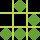
\includegraphics[width=\baselineskip,clip]{glider.png} 奥付}
\hrule\vskip.5mm\hrule\vskip3mm
\begin{tabular}{ll}
2015/8/15 & 初版発行\\
hash: & payo@payo(の次)\\
著作・発行 & NoNameA 774 (nonamea774@nnn77) \\
メールアドレス & \href{mailto:nonamea774@gmail.com}{\nolinkurl{nonamea774@gmail.com}}\\
Web & \url{https://nna774.net/}\\
Twitter & @nonamea774\\
GPG Key & 0x0C3E3AB2\\
fingerprint & 674A 287A 21D2 2431 AD8F \\
 & D328 AEF3 C3C7 0C3E 3AB2
\end{tabular}
\vskip3mm\hrule\vskip3mm

This article is licensed unser GFDL 1.3 or any later versions. And/or CC BY-SA 4.0 International.
You can get a machine-readable Transparent copy from \url{https://github.com/nna774/C88Paper}
\end{document}
